
\documentclass[a4paper,12pt]{article}
\usepackage{geometry}
\usepackage{amsmath}
\usepackage{array}
\usepackage{multicol}
\usepackage{fancyhdr}
\usepackage{listings}
\usepackage{xcolor}
\usepackage{tikz}
\usetikzlibrary{shapes.geometric, arrows.meta, positioning}

% Page setup
\geometry{margin=1in}
\pagestyle{fancy}
\fancyhf{}
\rhead{Functions \& Pointers in C}
\lhead{C Programming Notes}
\rfoot{\thepage}

% Code style
\lstset{
    language=C,
    basicstyle=\ttfamily\small,
    keywordstyle=\color{blue},
    commentstyle=\color{gray},
    stringstyle=\color{red},
    showstringspaces=false,
    frame=single,
    breaklines=true
}

% TikZ styles
\tikzset{
  flow/.style={draw, rounded corners=2pt, align=center, minimum width=3.8cm, minimum height=1.1cm},
  startstop/.style={flow, fill=black!5},
  process/.style={flow, fill=blue!5},
  decision/.style={flow, diamond, aspect=2, inner sep=1.2ex, fill=yellow!10},
  io/.style={flow, fill=green!7},
  danger/.style={flow, fill=red!8},
  arrow/.style={-Latex, line width=0.9pt}
}

\begin{document}

\begin{center}
    {\LARGE \textbf{Functions \& Pointers in C - Illustrated \vspace{0.3cm} [Notes]}} \\
    \vspace{0.5cm}
\end{center}

\section*{1. Function Basics}
Functions are reusable blocks of code that make programs modular and readable.  
\[
\text{Syntax: } return\_type \; function\_name(parameters) \; \{ \; body \; \}
\]

\textbf{Example:}
\begin{lstlisting}
int add(int a, int b) {
    return a + b;
}
\end{lstlisting}

\section*{2. Parameter Passing}
\textbf{Call by Value:} A copy of the argument is passed.  
\textbf{Call by Reference:} Using pointers, the function modifies the original variable.  

\section*{3. Pointers \& Memory Addressing}
- Declaration: \verb|int *p;|  
- Initialization: \verb|p = &x;|  
- Dereferencing: \verb|*p| accesses or modifies the value at the stored address.

\section*{4. Practical Example: Swap Function}
\begin{lstlisting}
void swap(int *a, int *b) {
    int temp = *a;
    *a = *b;
    *b = temp;
}
int main() {
    int x = 5, y = 10;
    swap(&x, &y);
    printf("%d %d", x, y); // Output: 10 5
}
\end{lstlisting}

\textbf{Memory Layout (before swap):}
\begin{verbatim}
   x = 5        y = 10
   +----+       +----+
   | 5  |       | 10 |
   +----+       +----+
     ^             ^
     |             |
     a             b
\end{verbatim}

\textbf{Memory Layout (after swap):}
\begin{verbatim}
   x = 10       y = 5
   +----+       +----+
   | 10 |       | 5  |
   +----+       +----+
     ^             ^
     |             |
     a             b
\end{verbatim}

\section*{5. Example: Pointer Dereferencing}
\begin{lstlisting}
int x = 42;
int *p = &x;

printf("%d", *p); // prints 42
\end{lstlisting}

\textbf{Memory Diagram:}
\begin{verbatim}
   +----+       +------+
   | 42 | <-- p | addr |
   +----+       +------+
      x
\end{verbatim}

\section*{6. Arrays and Pointers}
- An array name acts like a pointer to its first element.  
- Access: \verb|arr[i]| is equivalent to \verb|*(arr + i)|  

\begin{lstlisting}
int arr[3] = {10, 20, 30};
printf("%d", *(arr + 1)); // prints 20
\end{lstlisting}

\textbf{Memory Layout:}
\begin{verbatim}
   arr[0]     arr[1]     arr[2]
   +----+     +----+     +----+
   | 10 |     | 20 |     | 30 |
   +----+     +----+     +----+
     ^ 
     |
   arr or &arr[0]
\end{verbatim}

\section*{7. Dynamic Memory Allocation (Intro)}
Pointers allow creation of memory at runtime.  

\begin{lstlisting}
int *ptr;
ptr = (int*) malloc(3 * sizeof(int));

ptr[0] = 5;
ptr[1] = 15;
ptr[2] = 25;

free(ptr); // release memory
\end{lstlisting}

\section*{8. Linked List Basics}
A linked list is a collection of nodes, where each node contains data and a pointer to the next node.  

\begin{lstlisting}
struct Node {
    int data;
    struct Node *next;
};

int main() {
    struct Node n1, n2, n3;

    n1.data = 10; n1.next = &n2;
    n2.data = 20; n2.next = &n3;
    n3.data = 30; n3.next = NULL;

    struct Node *head = &n1;
    while(head != NULL) {
        printf("%d -> ", head->data);
        head = head->next;
    }
}
\end{lstlisting}

\textbf{Memory Diagram:}
\begin{verbatim}
   +------+     +------+     +------+
   | 10   | --> | 20   | --> | 30   | --> NULL
   +------+     +------+     +------+
\end{verbatim}

\section*{9. Common Pointer Errors}
\subsection*{a) Uninitialized Pointer}
\begin{lstlisting}
int *p;     // uninitialized
*p = 5;     // ERROR: random memory location
\end{lstlisting}

\subsection*{b) Dangling Pointer}
\begin{lstlisting}
int *p = (int*) malloc(sizeof(int));
free(p);
*p = 10;    // ERROR: using freed memory
\end{lstlisting}

\subsection*{c) NULL Pointer Dereference}
\begin{lstlisting}
int *p = NULL;
printf("%d", *p); // ERROR: segmentation fault
\end{lstlisting}

\subsection*{d) Array Out of Bounds}
\begin{lstlisting}
int arr[3] = {1,2,3};
printf("%d", arr[5]); // ERROR: invalid memory access
\end{lstlisting}

\subsection*{e) Multiple Free}
\begin{lstlisting}
int *p = (int*) malloc(sizeof(int));
free(p);
free(p);  // ERROR: double free
\end{lstlisting}

\section*{10. Why Pointers Matter}
- Dynamic memory management  
- Efficient array and string handling  
- Building data structures (linked lists, trees)  
- Direct hardware/memory access  

\section*{11. Best Practices}
- Always initialize pointers before use  
- Avoid dangling pointers  
- Set to \verb|NULL| after \verb|free|  
- Check if \verb|malloc| returned \verb|NULL|  
- Free dynamically allocated memory  

\section*{12. Summary Table}
\renewcommand{\arraystretch}{1.3}
\begin{tabular}{|m{4cm}|m{9cm}|}
\hline
\textbf{Concept} & \textbf{Description} \\
\hline
Function Declaration & \verb|return_type name(params);| defines a function \\
\hline
Call by Value & Copies arguments; original variables unchanged \\
\hline
Pointers \& References & Use addresses to directly modify original variables \\
\hline
Swapping via Pointers & Example using \verb|swap(int *a, int *b)| \\
\hline
Arrays and Pointers & \verb|arr[i] == *(arr+i)| \\
\hline
Dynamic Memory Allocation & \verb|malloc, calloc, realloc, free| \\
\hline
Linked List Basics & Nodes linked via \verb|next| pointers \\
\hline
Pointer Errors & Uninitialized, dangling, NULL deref, OOB, double free \\
\hline
Pointer Safety & Initialize, check, free, nullify \\
\hline
\end{tabular}

\section*{13. TikZ Flowchart: Pointer Lifecycle}
\begin{center}
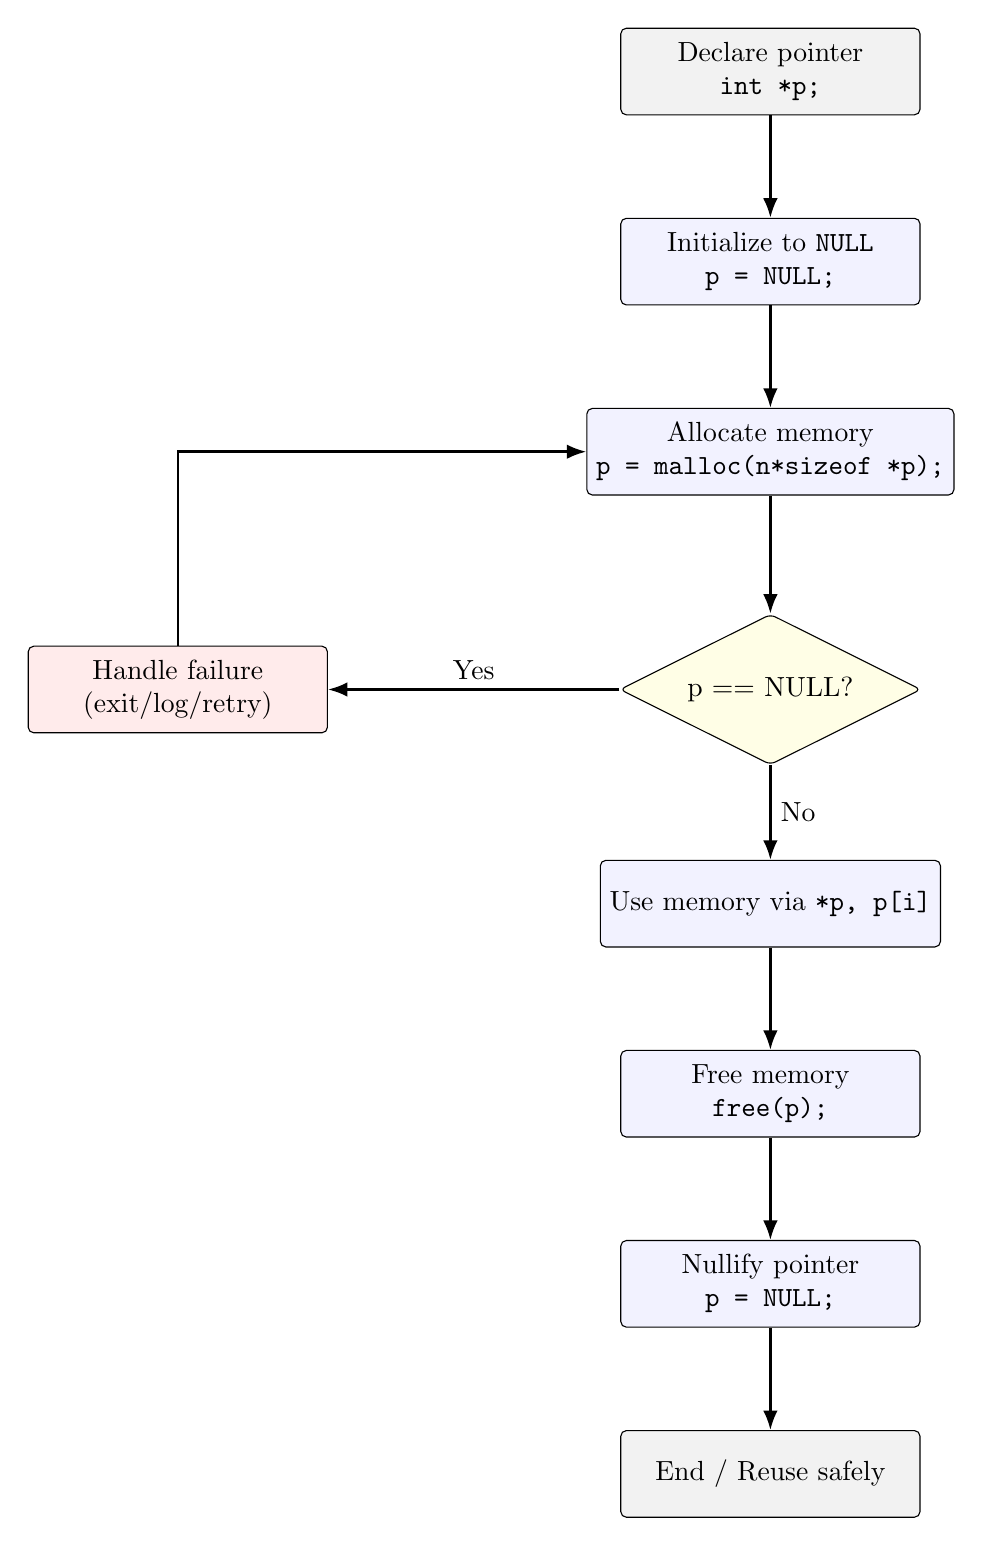
\begin{tikzpicture}[node distance=1.3cm]
  % Nodes
  \node[startstop] (start) {Declare pointer\\ \verb|int *p;|};
  \node[process, below=of start] (init) {Initialize to \verb|NULL|\\ \verb|p = NULL;|};
  \node[process, below=of init] (alloc) {Allocate memory\\ \verb|p = malloc(n*sizeof *p);|};
  \node[decision, below=of alloc, yshift=-2mm] (check) {p == NULL?};
  \node[danger, left=3.7cm of check] (handle) {Handle failure\\ (exit/log/retry)};
  \node[process, below=1.2cm of check] (use) {Use memory via \verb|*p, p[i]|};
  \node[process, below=of use] (free) {Free memory\\ \verb|free(p);|};
  \node[process, below=of free] (nullify) {Nullify pointer\\ \verb|p = NULL;|};
  \node[startstop, below=of nullify] (end) {End / Reuse safely};

  % Arrows
  \draw[arrow] (start) -- (init);
  \draw[arrow] (init) -- (alloc);
  \draw[arrow] (alloc) -- (check);
  \draw[arrow] (check.west) -- node[above]{Yes} (handle.east);
  \draw[arrow] (handle.north) |- (alloc.west);
  \draw[arrow] (check) -- node[right]{No} (use);
  \draw[arrow] (use) -- (free);
  \draw[arrow] (free) -- (nullify);
  \draw[arrow] (nullify) -- (end);
\end{tikzpicture}
\end{center}

\end{document}
